\chapter{Background}\label{ch:Background}

People create all sorts of digital content in a variety of formats and on a massive scale. Regardless of how information is shaped, we—as humans—are capable of extracting the inherent semantics by inferring implicit knowledge about a given information. For example, a piece of information represented in a textual form is: \textit{The marble is white}. We probably understand the meaning of that statement, as we know that marble refers to a material and white to a color. Even though this additional information was not provided explicitly to us, we can infer that knowledge implicitly, to understand the meaning of the statement. In addition to this one possible meaning, however, this sentence may also refer to a toy:~a~marble. Ultimately, the context in which this statement is embedded would resolve this ambiguity for a human reader. Nevertheless, this example demonstrates the way we link information. In fact, our brain consists of neurons (analogous to graph nodes) interconnected by synapses (analogous to graph edges), creating a neural network, which is a complex graph structure \parencite[1]{Stanley2013}. Linking, interpreting, and evaluating information may seem trivial to us since our brain has evolved to perform cognitively demanding tasks on a daily basis. For a computer, in contrast, understanding semantics is a complex task, as it is not capable of inferring knowledge by default. Making a computer understand (especially ambiguous) semantics thus represents a  challenging endeavor. 


\section{Semantic Web}\label{sec:Semantic Web}

The research field \textit{Semantic Web} (or \textit{Linked Data}) aims to address the previous matter. The basic idea is to enrich information with resource identifiers that link to a distinct entry in a catalog (i.e., a vocabulary/ontology\footnote{Disambiguation of vocabulary and ontology:\enspace{}\textit{``There is no clear division between what is referred to as `vocabularies' and `ontologies'. The trend is to use the word `ontology' for more complex, and possibly quite formal collection of terms, whereas `vocabulary' is used when such strict formalism is not necessarily used or only in a very loose sense. Vocabularies are the basic building blocks for inference techniques on the Semantic Web.''} \parencite{W3COntologies}}). This link allows computers (and humans) to understand what a resource is referring to. There is no need to provide more context, as linked data grants semantic uniqueness by design. Linked data uses the graph-based \acrfull*{RDF} as the underlying data model, which broadly describes the relationship between resources \mbox{\parencite{RDF1997}.}

An \acrshort*{RDF} graph consists of three components, which can be expressed as a semantic triple: \textit{subject-predicate-object}. To illustrate the previous statement, the semantic triple for white marble would translate to \textit{marble-hasColor-white}. In \acrshort*{RDF}, the subject designates a specific resource (e.g., \textit{marble}), while the predicate denotes a specific property of that subject (e.g., \textit{hasColor)}. Furthermore, a predicate describes the relation between a subject and an object. However, depending on the domain and the language being used in this field, there are different ways to express a triple. While some authors (e.g., \cite[115]{Fensel2005} and \cite[581]{Khosrow2006}) refer to \textit{object-property-value} triples, the \tracknshrink{EAV} model expresses \acrshort*{RDF} as an \textit{entity-attribute-value} triple. \textcite[17]{Powers2003} concludes that


\begin{displayquote}
\hspace*{-1.4mm}``[\textellipsis{}] simple facts can almost always be defined given three specific pieces of information: the subject of the fact, the property of the subject that is currently being defined, and its associated value. This correlates to what we understand to be a complete thought, regardless of differing syntaxes based on language.''
\end{displayquote}

\noindent Subjects and predicates always use a resource identifier (i.e., a \acrshort*{URI}/\acrshort*{IRI})\footnote{Throughout this work, I will interchangeably use both abbreviations \acrshort*{URI} (\acrlong*{URI}) and \acrshort*{IRI} (\acrlong*{IRI}). The latter extends the characters in \tracknshrink{URIs} from a subset of the \tracknshrink{ASCII} character set to almost all characters of the Universal Character Set (Unicode/\tracknshrink{ISO} 10646).} to describe their exact entity and property. Objects, on the other hand, may either refer to a \acrshort*{URI} as well or to a (string) literal.\footnote{In \acrshort*{RDF} objects (and thus subjects) may also be a blank node; however, this has no further relevance for this work.}
To disambiguate the marble example, \tracknshrink{URIs} can be used to express the meaning distinctly, which was demonstrated in the previous chapter (Introduction) in \autoref{lst:MinimalGraph}, where the \tracknshrink{URI} referred to marble as a material and not the toy.

As stated, \acrshort*{RDF} intrinsically represents a graph structure. Moreover, it is a \textit{``[\textellipsis{}] good example of a labeled directed multigraph [\textellipsis{}]''} \parencite[21]{Shaposhnik2015}. To illustrate this concept, \autoref{fig:White Marble Graph Extended} depicts a graph expressing the geological classification of the material marble.

\begin{figure}[ht]
    \libertineLF
    \centering
    

\tikzset{every picture/.style={line width=0.75pt}} %set default line width to 0.75pt        

\begin{tikzpicture}[x=0.75pt,y=0.75pt,yscale=-1,xscale=1]
%uncomment if require: \path (0,182); %set diagram left start at 0, and has height of 182

%Shape: Ellipse [id:dp24670974058563444] 
\draw  [draw opacity=0][fill={rgb, 255:red, 104; green, 139; blue, 181 }  ,fill opacity=1 ][blur shadow={shadow xshift=0pt,shadow yshift=-2.25pt, shadow blur radius=1.5pt, shadow blur steps=4 ,shadow opacity=25}] (199.4,25) .. controls (199.4,12.79) and (225.03,2.89) .. (256.65,2.89) .. controls (288.27,2.89) and (313.9,12.79) .. (313.9,25) .. controls (313.9,37.21) and (288.27,47.11) .. (256.65,47.11) .. controls (225.03,47.11) and (199.4,37.21) .. (199.4,25) -- cycle ;

%Straight Lines [id:da9585060066991378] 
\draw [color={rgb, 255:red, 104; green, 139; blue, 181 }  ,draw opacity=1 ][line width=3]    (256.65,52.11) -- (326.61,122.08) ;
\draw [shift={(330.15,125.61)}, rotate = 225] [fill={rgb, 255:red, 104; green, 139; blue, 181 }  ,fill opacity=1 ][line width=3]  [draw opacity=0] (18.75,-9.01) -- (0,0) -- (18.75,9.01) -- (12.45,0) -- cycle    ;

%Shape: Ellipse [id:dp08840031080406163] 
\draw  [draw opacity=0][fill={rgb, 255:red, 104; green, 139; blue, 181 }  ,fill opacity=1 ][blur shadow={shadow xshift=0pt,shadow yshift=-2.25pt, shadow blur radius=1.5pt, shadow blur steps=4 ,shadow opacity=25}] (304.4,147) .. controls (304.4,134.3) and (338.54,124) .. (380.65,124) .. controls (422.76,124) and (456.9,134.3) .. (456.9,147) .. controls (456.9,159.7) and (422.76,170) .. (380.65,170) .. controls (338.54,170) and (304.4,159.7) .. (304.4,147) -- cycle ;

%Straight Lines [id:da8093278208429049] 
\draw [color={rgb, 255:red, 104; green, 139; blue, 181 }  ,draw opacity=1 ][line width=3]    (256.65,52.11) -- (199.83,121.14) ;
\draw [shift={(196.65,125)}, rotate = 309.46000000000004] [fill={rgb, 255:red, 104; green, 139; blue, 181 }  ,fill opacity=1 ][line width=3]  [draw opacity=0] (18.75,-9.01) -- (0,0) -- (18.75,9.01) -- (12.45,0) -- cycle    ;

%Shape: Rectangle [id:dp40317210341485543] 
\draw  [draw opacity=0][fill={rgb, 255:red, 104; green, 139; blue, 181 }  ,fill opacity=1 ][blur shadow={shadow xshift=0pt,shadow yshift=-2.25pt, shadow blur radius=1.5pt, shadow blur steps=4 ,shadow opacity=25}] (140,128.99) -- (253.9,128.99) -- (253.9,165) -- (140,165) -- cycle ;

%Shape: Ellipse [id:dp29246590127054906] 
\draw  [draw opacity=0][fill={rgb, 255:red, 104; green, 139; blue, 181 }  ,fill opacity=1 ][blur shadow={shadow xshift=0pt,shadow yshift=-2.25pt, shadow blur radius=1.5pt, shadow blur steps=4 ,shadow opacity=25}] (375.4,25) .. controls (375.4,11.75) and (411.33,1) .. (455.65,1) .. controls (499.97,1) and (535.9,11.75) .. (535.9,25) .. controls (535.9,38.25) and (499.97,49) .. (455.65,49) .. controls (411.33,49) and (375.4,38.25) .. (375.4,25) -- cycle ;

%Straight Lines [id:da3097512749321867] 
\draw [color={rgb, 255:red, 104; green, 139; blue, 181 }  ,draw opacity=1 ][line width=3]    (383.65,121) -- (449.11,55.54) ;
\draw [shift={(452.65,52)}, rotate = 495] [fill={rgb, 255:red, 104; green, 139; blue, 181 }  ,fill opacity=1 ][line width=3]  [draw opacity=0] (18.75,-9.01) -- (0,0) -- (18.75,9.01) -- (12.45,0) -- cycle    ;


% Text Node
\draw (256.65,25) node [scale=1.2] [align=left] {{\textsf{\textbf{:Marble}}}};
% Text Node
\draw (380.65,147) node [scale=1.2] [align=left] {{\footnotesize {\textsf{\textbf{:Metamorphic\_rock}}}}};
% Text Node
\draw (196.95,147) node  [align=left] {{\textsf{\textbf{"Marmor"@de}}}};
% Text Node
\draw (455.65,25) node [scale=1.2] [align=left] {{\textsf{\textbf{:Rock\_(geology)}}}};
% Text Node
\draw (223.9,77.09) node [scale=0.7,rotate=-309] [align=left] {{\textsf{\textbf{rdfs:label}}}};
% Text Node
\draw (298.4,82.09) node [scale=0.7,rotate=-45] [align=left] {{\textsf{\textbf{rdfs:subClassOf}}}};
% Text Node
\draw  [draw opacity=0]  (368.75,49.95) -- (442.05,49.95) -- (442.05,123.24) -- (368.75,123.24) -- cycle  ;
\draw (405.4,86.59) node [scale=0.7,rotate=-315] [align=left] {{\textsf{\textbf{rdfs:subClassOf}}}};


\end{tikzpicture}

	\caption[A Labeled Directed \acrshort*{RDF} Multigraph]{A labeled directed \acrshort*{RDF} multigraph, expressing the broader classification of the material marble, and stating marble’s (German) label as an annotated object literal.}
	\label{fig:White Marble Graph Extended}
	\libertineOsF{}
\end{figure}

\noindent In a directed (\acrshort*{RDF}) graph, arrows are reflecting the graph’s directional nature, and objects, as illustrated, may refer to other resources, creating new semantic triples. These features do not only allow \acrshort*{RDF} to describe logical relations between things but also to create complex frameworks working on top of it. Relevant for this work are frameworks defining a syntax, structure, or shape (e.g., \acrshort*{RDFS},\footnote{Resource Description Framework Schema by \cite{RDFS1999}} \acrshort*{OWL},\footnote{Web Ontology Language by \cite{OWL2004}} \acrshort*{SHACL},\footnote{Shapes Constraint Language by \cite{SHACL2015}} or different vocabularies/ontologies defining specific terms (e.g., \acrshort*{FOAF},\footnote{Friend Of A Friend by \cite{Miller2014}} \tracknshrink{DCT},\footnote{Dublin Core Metadata Terms by the \cite{DublinCoreTerms}} etc.).

A notable application in the field of linked data is DBPedia \parencite{DBpedia2009}, which extracts structured information from the Wikipedia project and allows users to query this information. Similar to the preceding examples of graph data, \autoref{lst:WhiteMarbleSubClassOf} is using resources referring to DBPedia. The following code is representing \autoref{fig:White Marble Graph Extended} in Turtle notation.\footnote{Code listings in this work are omitting the prefix notation shared by N3, Turtle, and \acrshort*{SPARQL}. In the digital version of this work, clicking a prefixes will link to the corresponding \acrshort*{IRI} on page \pageref{ch:LOA} at the beginning of this work.}

\begin{spacing}{0.9}
  \lstset{language=JavaScript,escapechar=|}
  \begin{lstlisting}[
  label={lst:WhiteMarbleSubClassOf},
  xleftmargin=15em, % this needs to be manually adjusted to center the frame
  xrightmargin=-15em, % this needs to be manually adjusted to center the frame
  caption={[A Minimal Graph in Turtle Notation]A minimal graph in Turtle notation representing \autoref{fig:White Marble Graph}.}]
|<\url{http://dbpedia.org/resource/Marble}>|
  |\acrshort{rdfs}|subClassOf
    |<\url{http://dbpedia.org/resource/Metamorphic\_rock}> ;|
  |\acrshort{rdfs}|label "Marmor"@de .
|<\url{http://dbpedia.org/resource/Metamorphic\_rock}>|
  |\acrshort{rdfs}|subClassOf
    |<\url{http://dbpedia.org/resource/Rock\_(geology)}> .
\end{lstlisting}
\end{spacing}




\newpage



\section{Kanban}\label{sec:Kanban}

The Kanban system was invented by Taiichi Ohno, an industrial engineer at Toyota in 1947. It establishes a just-in-time method of inventory control.
The word Kanban, in its literal translation (jap. {\footnotesize \begin{CJK}{UTF8}{min}看\,板\end{CJK}}), describes a cardboard, which represents one of the core components of the Kanban system.

In general, a \textit{Kanban board} visualizes work in progress (\tracknshrink{WIP}) items that are referred to as \textit{cards} on the board.
In most scenarios, cards are flowing from left to right over the \textit{columns} of a board, indicating their current stage of progress.
Boards may also be divided into horizontal \textit{swimlanes} (or just \textit{lanes}), which add another container to categorize groups of cards (e.g., different teams performing the work).

\subsection{Board Anatomy}

\autoref{fig:Kanban Boards} illustrates the evolving stages of a Kanban board by gradually adding more features to the first board (A). While all boards share the same three labels for their columns (i.e., \textit{ToDo}, \textit{Doing}, \textit{Done}), they differ in their card and lane structure. In particular, board (A) consists of five cards, board (B1) adds three more cards that belong to another domain or \textit{class}, and lastly, board (B2) extends (B1) by separating the cards into their classes using swimlanes (i.e., \textit{Box X} and \textit{Box Y}).


\begin{figure}[ht]
	\centering \begin{tikzpicture}
	\node[anchor=south west,inner sep=0] (image) at (0,0,0) {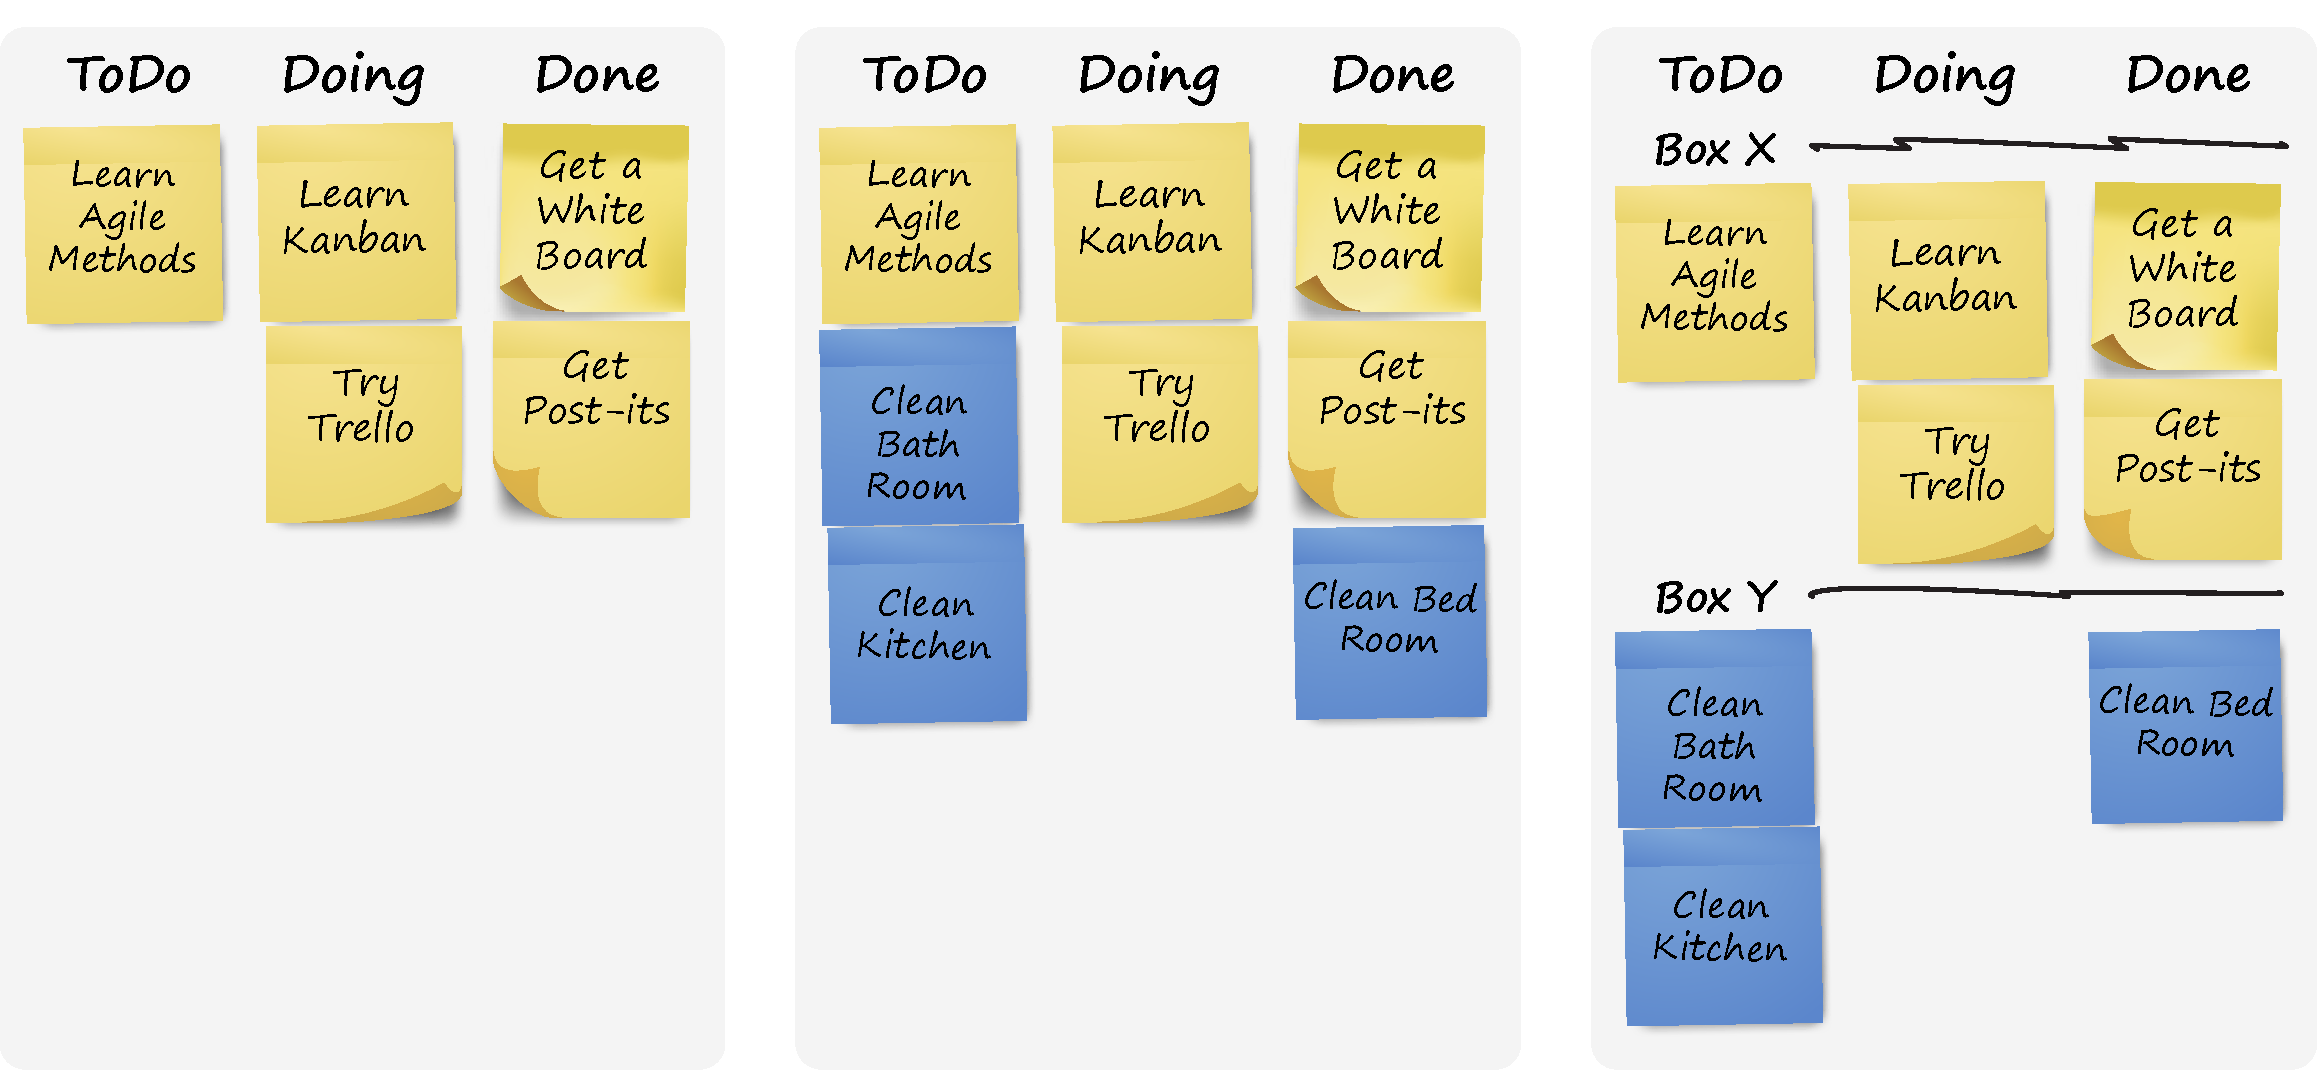
\includegraphics[width=\linewidth]{img/draw-kanban.pdf}};
	\begin{scope}[x={(image.south east)},y={(image.north west)}]
% 	% next four lines will help you to locate the point needed by forming a grid. comment these four lines in the final picture.↓
% 		\draw[help lines,xstep=.05,ystep=.05] (0,0) grid (1,1);
% 		\draw[help lines,xstep=.05,ystep=.05] (0,0) grid (1,1);
% 		\foreach \x in {0,1,...,9} { \node [anchor=north] at (\x/10,0) {0.\x}; }
% 		\foreach \y in {0,1,...,9} { \node [anchor=east] at (0,\y/10) {0.\y};}
% 	% upto here↑
	

	
	\draw (0.155,1.020) node {(A)};
	\draw (0.498,1.020) node {(B1)};
	\draw (0.842,1.020) node {(B2)};
	
	\end{scope}
	\end{tikzpicture}
	\caption[Three Examples of a Kanban Board]{Three examples of a Kanban board, with different board components (i.e., cards, columns, and lanes). Cards are depicted by post-it notes. Board (B1) contains cards with mixed classes, board (B2) is separating card classes using swimlanes (i.e., \textit{Box X} and \textit{Box Y}).}
	\label{fig:Kanban Boards}
\end{figure}



\noindent There are two perspectives on how a Kanban board can be conceptualized, that is (1) by their \textit{board component resources} and (2) \textit{card component resources}. Both perspectives will be repeatedly referenced throughout this work.

\textbf{Board component resources} refer to the \textit{class} of each structural component (i.e., cards, columns, and lanes). In other words, it refers to the origin of each board component. For example, in board (A) in \autoref{fig:Kanban Boards}, all the post-it notes may be stored in a storage box labeled \textit{Box X}. This storage box would represent the \textit{class} of the cards. Principally, one board can carry cards from multiple classes. For example, a second storage box labeled \textit{Box Y} could contain various post-it notes referring to a different class. Board (B1), as depicted in \autoref{fig:Kanban Boards}, provides an example of a board keeping track of two classes: a person’s cleaning progress and their Kanban achievements. Both classes fit the semantics of the board columns (\kern1pt\tracknshrink{|\,\textit{ToDo}\,|\,\textit{Doing}\,|\,\textit{Done}\,|}\kern1pt). However, when using multiple card classes, it may be helpful to clearly separate cards into their classes by using swimlanes, as depicted by board (B2).

In contrast to cards, columns and lanes typically have one single class each. The column labels in \autoref{fig:Kanban Boards}, for example, could belong to a storage box labeled \textit{Basic ToDo Progress Labels}. Let us assume that one would like to add another box, labeled \textit{Weekplaner} containing column labels ranging from Monday to Friday, containing column labels ranging from Monday to Friday. Merging both classes \textit{Basic ToDo Progress Labels} and \textit{Weekplanner} would require a more complex (three-dimensional or nested) board solution, lacking in user-friendliness and applicability. 

\textbf{Card component resources} refer to the resources that are depicted on a card (i.e., their content). Compared to the tight boundaries of board component resources, card component resources are virtually endless regarding the number of displayable elements. The text on the post-it notes in \autoref{fig:Kanban Boards}, for example, can be considered as the card’s title resource. Principally, cards may further depict a descriptive text, a due date, a creation date, or the name of an assignee.


\subsection{General Board Usage}

Building upon the idea of the traditional paper-pencil boards (e.g., \autoref{fig:Kanban Boards}), a variety of digital Kanban solutions have been developed.\footnote{Wikipedia lists some examples: \url{https://en.wikipedia.org/wiki/Kanban_board\#Notable_tools}.} Even though these solutions vary in their scope and price models, they all share a basic feature set: Most apparent, all solutions allow users to create cards and columns from scratch. Furthermore, cards contain at least a title and may also have a description field to provide more context to the user. Lastly, by definition, cards can be moved from one column to another to indicate their current stage of progress.

Due to the vast array of application fields (e.g., personal task management, marketing teams, human resources, etc.), there are countless ways to design a Kanban board. Notably, in the field of agile software development, Kanban had a particularly strong impact over the last two decades \parencite[11]{Stoica2016}.

Over the course of a project, a Kanban board has the potential to grow in complexity (i.e., more cards, columns, and lanes). There are established principles to maintain a lean state to tackle this case. Two of the most prominent are: (1) define a maximum card limit for a board to prevent your team from exceeding their capacity, and (2) \textit{walk the board} from right to left. That means although cards usually flow from left to right, \textit{“[\textellipsis{}] you iterate over the tickets from right to left: Closest to completion to most recently started.”} \parencite{Anderson2016}. 

Nevertheless, in this work, the Kanban board is used to visualize a section of an existing \acrshort*{RDF} graph and to mutate a specific value by relocating cards on the board. In other words, and in contrast to most Kanban applications, the focus is not on creating \acrshort*{RDF} resources within the board, but on visualizing and managing existing ones. Note that throughout this thesis, I will use the terms \textit{resource} and \textit{card} interchangeably, since---in this shared context---a card always refers to an \acrshort*{RDF} resource. For example, the \textit{DBpedia} entry for marble is a resource and thus a card in the board, as illustrated in \autoref{fig:White Marble Kanban Board}.


